\section{Databasen}
\label{Technical_Database}

\subsection{Kravspecifikationens datamodel}
\label{Technical_Database_ks}
Kravspecifikationens kapitel \textit{D} \cite[s.14]{kravspec} præsenterer følgende model for det data, systemet skal bruge:
\begin{figure}[h!]
  \centering
    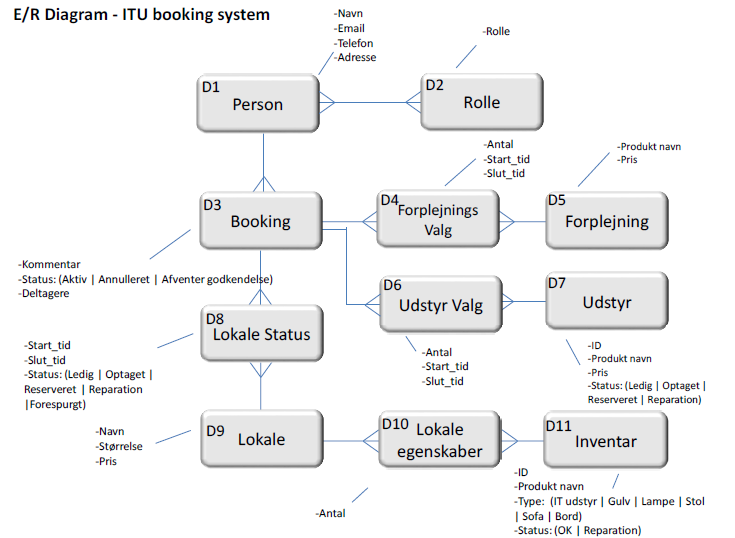
\includegraphics[width=\textwidth]{Chapters/Design/Technical/Images/KSdata}
  \caption{Kravspecifikationens datamodel}
\label{Fig:Technical_Database_ks_KSdata}
\end{figure}

Der er en række ting, som skal ændres ved datamodellen for at tilpasse den til vores løsning. 

\subsubsection{Personinformation}
\label{Technical_Database_ks_personinfo}
Det har primært været vores fokus at understøtte anvendelsen af IT-Universitetets Active Directory (AD) til at logge ind i systemet. Da ITUs AD ikke indeholder addresse eller telefonnummer, så inkluderer vi det ikke i vores datamodel. Dette kunne eventuelt indføres senere, hvis man ændrede i AD, brugte et andet system til godkende adgang eller lod brugeren redigere i sine data.

\subsubsection{Priser på lokaler/udstyr}
\label{Technical_Database_ks_prices}
Vi har valgt ikke at understøtte eksterne brugere i første release, er det ikke nødvendigt at inkludere priser på lokaler og udstyr. De kunne eventuelt blive introduceret som separate entiteter i databaser, således at priser kan justeres efter hvilken rolle, brugeren har i systemet.

\subsubsection{Lokale status}
\label{Technical_Database_ks_roomStatus}
Vi besluttede os for, at en booking kun kan bestå af et enkelt tidsrum og et enkelt lokale. Dette var hovedsageligt for at gøre det nemmere at implementere. Det gør det dog også nemmere at design brugergrænsefladen, da man ikke behøver lave et nyt skærmbillede i forbindelse med ændring af lokaler/tid til en booking.

\subsubsection{Lokale egenskaber}
\label{Technica l_Database_ks_roomProperties}
Da vi vil bruge 7

\subsubsection{Inventar- og udstyrstyper}
\label{Technical_Database_ks_types}

\subsubsection{Udstyr}
\label{Technical_Database_ks_eChoice}

\subsubsection{Forplejning}
\label{Technical_Database_ks_catering}

\subsection{Vores datamodel}
\label{Technical_Database_our}

Kravspecifikationens kapitel \textit{D} \cite[s.14]{kravspec} præsenterer følgende model for det data, systemet skal bruge:
\begin{figure}[h!]
  \centering
    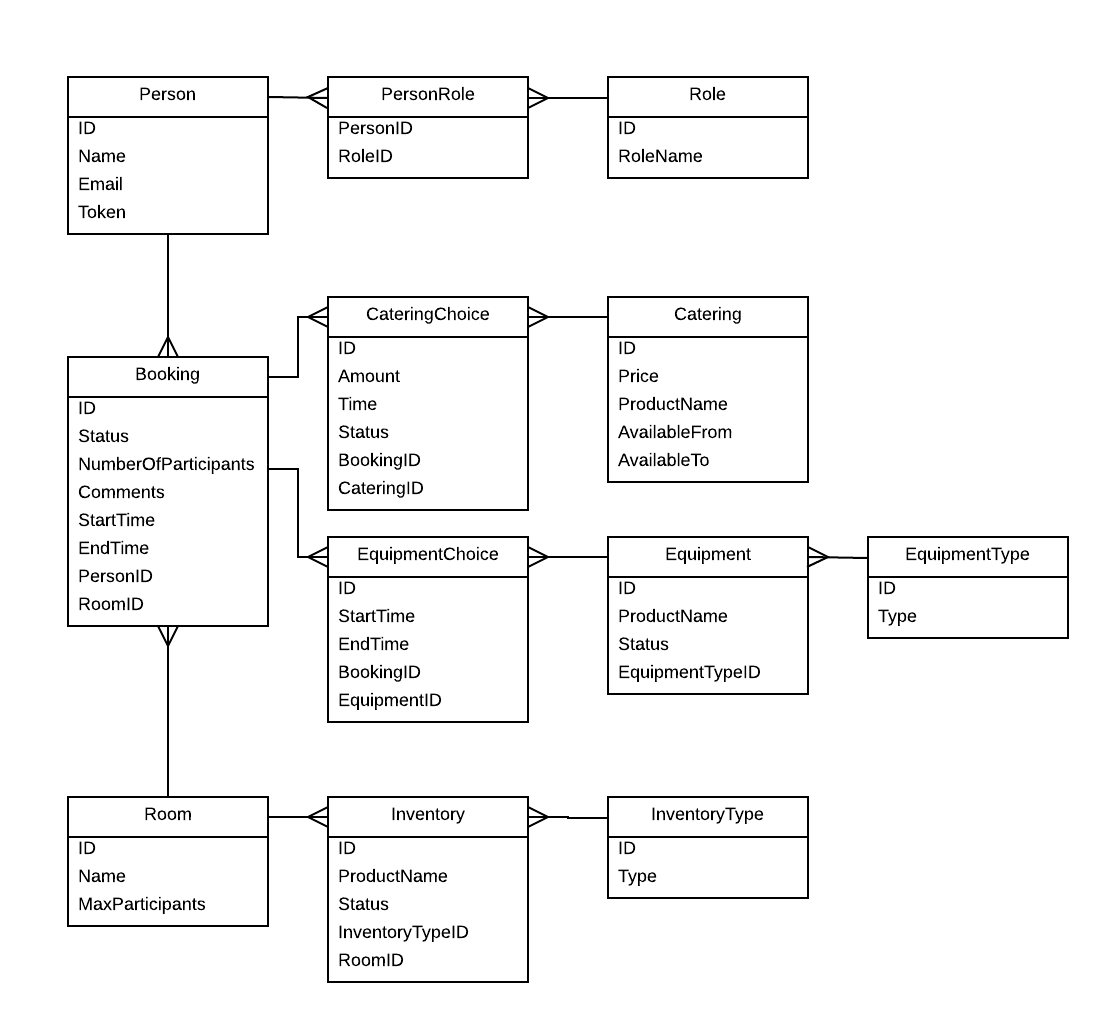
\includegraphics[width=\textwidth]{Chapters/Design/Technical/Images/OurDataModel}
  \caption{Datamodellen til vores løsning}
\label{Fig:Technical_Database_our_datamodel}
\end{figure}